\documentclass[10pt,conference]{IEEEtran}

\ifCLASSINFOpdf
	\usepackage[pdftex]{graphicx}
	\graphicspath{{./figs/}}
	\DeclareGraphicsExtensions{.pdf,.jpeg,.png}
\else
	\usepackage[dvips]{graphicx}
	\graphicspath{{./figs/}}
	\DeclareGraphicsExtensions{.eps}
\fi

\usepackage[cmex10]{amsmath}
\usepackage[tight,footnotesize]{subfigure}

\usepackage{xcolor}
\usepackage[lined,ruled]{algorithm2e}

\usepackage[latin1]{inputenc}
\usepackage{tikz}
\usetikzlibrary{shapes}
\usetikzlibrary{arrows}

\usepackage[]{algorithm2e}

\newtheorem{property}{Property}
\newtheorem{proposition}{Proposition}
\newtheorem{theorem}{Theorem}
\newtheorem{conjecture}{Conjecture}
\newtheorem{question}{Question}
\newtheorem{definition}{Definition}
\newtheorem{corollary}{Corollary}

\makeatletter
\pgfdeclareshape{datastore}{
  \inheritsavedanchors[from=rectangle]
  \inheritanchorborder[from=rectangle]
  \inheritanchor[from=rectangle]{center}
  \inheritanchor[from=rectangle]{base}
  \inheritanchor[from=rectangle]{north}
  \inheritanchor[from=rectangle]{north east}
  \inheritanchor[from=rectangle]{east}
  \inheritanchor[from=rectangle]{south east}
  \inheritanchor[from=rectangle]{south}
  \inheritanchor[from=rectangle]{south west}
  \inheritanchor[from=rectangle]{west}
  \inheritanchor[from=rectangle]{north west}
  \backgroundpath{
    %  store lower right in xa/ya and upper right in xb/yb
    \southwest \pgf@xa=\pgf@x \pgf@ya=\pgf@y
    \northeast \pgf@xb=\pgf@x \pgf@yb=\pgf@y
    \pgfpathmoveto{\pgfpoint{\pgf@xa}{\pgf@ya}}
    \pgfpathlineto{\pgfpoint{\pgf@xb}{\pgf@ya}}
    \pgfpathmoveto{\pgfpoint{\pgf@xa}{\pgf@yb}}
    \pgfpathlineto{\pgfpoint{\pgf@xb}{\pgf@yb}}
 }
}
\makeatother

\newcommand{\riham}[1]{{\color{red}{#1}}}
\newcommand{\james}[1]{{\color{blue}{#1}}}


\begin{document}

\title{CS-336 Project 2015: Hardware Parts}
\author{
\IEEEauthorblockN{Matthew Eder}
\IEEEauthorblockA{Rutgers University\\ 
Piscataway, NJ, USA\\
Email: mre56@scarletmail.rutgers.edu}
\and
\IEEEauthorblockN{Michael Azzimaro}
\IEEEauthorblockA{Rutgers University\\
Piscataway, NJ, USA\\
Email: michazzi@scarletmail.rutgers.edu}
\and
\IEEEauthorblockN{Michael Calabrese}
\IEEEauthorblockA{Rutgers University\\
Piscataway, NJ, USA\\
Email: mrcalabrese2@gmail.com}
}


\maketitle


\begin{abstract}
\textnormal{
In this project, we intend to build a computer hardware Data Base Management System from the ground up that composes of multiple stages. The database system will be used for the sole purpose of immersing its users with computer hardware data. The overall project begins with stage one, which is intended for analyzing how specific users of the computer hardware database interact with the database environment.  Stage two will bring stage one to life through a use of a pictorial design of the computer hardware database system. Here, an ER model will be presented as a means of describing relations between entities of the computer hardware database system. Also stated in this report is stage three, describing how we intend to lay out our database design through the use of SQL tables. Finally, stage four will describe the User Interface that will be based off of the computer hardware database system design. Overall, this project seeks to build a computer hardware database system for multiple user types. We intend to design and implement a computer hardware database system that encourages easy accessibility and maneuverability for its users. 
}
\end{abstract}
%\onecolumn \maketitle \normalsize \vfill

\IEEEpeerreviewmaketitle
 %%%%%%%%%%%%%%%%%%%%%%%%%%%%%%%%%%%%%%%%%%%%%%%%%%%%%%%%%%%%%%%%%%%%%%%%%%%%%%%%%%%%%%%%%%%%%%%%%%%%%%%%%
%\section{Project Description}\label{sec:1. Project Description}
%\input{introduction.tex}
%%%%%%%%%%%%%%%%%%%%%%%%%%%%%%%%%%%%%%%%%%%%%%%%%%%%%%%%%%%%%%%%%%%%%%%%%%%%%%%%%%%%%%%%%%%%%%%%%%%%%%%%%
%\textnormal{
%Insert your project here.You can refer to the Abstract of the 336ProjectDescriptionSummer2015 LaTeX file as an example.
%The project has four stages, as follows.
%}
\subsection{Stage1 - The Requirement Gathering Stage. }\label{sec:1.	Requirement Gathering Stage. }
%%%%%%%%%%%%%%%%%%%%%%%%%%%%%%%%%%%%%%%%%%%%%%%%%%%%%%%%%%%%%%%%%%%%%%%%%%%%%%%%%%%%%%%%%%%%%%%%%%%%%%%%%%
\textnormal{
%\begin{itemize} 
%\item{}
%\end{itemize}
\begin{itemize} 
\item{The general system description: }
\textnormal{
This is a database of computer hardware parts and detailed information about those parts. The goal of this is to simplify part comparisons.  Parts have multiple filterable categories to allow easy and quick access when comparing a large number of parts.  By acting as a selection guide this database could be used to assist people to build there own computers.  There are four different types of users in this database manufactures, sellers, account users and guest users.
}
\item{The 4 types of users (grouped by their data access/update rights): }
\begin{itemize} 
\item{The user's access rights: }
The four types of users for our database include the manufacturer, the seller, account customers and guest users. The manufacturers main purpose is to update the database, detailing new product information as well as release dates on their respective computer hardware. Out of all users of the database, manufacturers are allowed the most data access and update rights. Specifically, manufactures are permitted to add new data to the database as well as remove previously added information respectively. Different manufactures cannot alter computer hardware information that is not their own. Additionally, manufacturers are allowed read access to account-customer reviews. \\ The sellers will compose of a variety of different online retailers for computer hardware parts. The seller's main contribution to the database is to list product prices as well as provide computer hardware specifications that are provided by the manufacturer. The seller will be allowed data access to all manufacture products. Sellers will also be allowed to group hardware parts into categories based on its purpose and functionality. As a way of receiving feedback from customers, sellers will also be granted the ability to create a customer reviews section on the respective product page. As compared to manufactures, sellers are limited when it comes to update rights. No seller is permitted to alter computer hardware product information unless authorized by the manufacturer themselves. Additionally, sellers are not allowed to modify and/or delete account-customer reviews unless the content of the review pertains no correspondence to the product whatsoever. \\Account users can access the prices of a specific grouping of hardware pieces, they can also get seller information based on location and price.  Account users also gain read access to the manufacturer information and the specifications of the products. They also gain read and write access to reviews of those products with the ability to rate and write reviews. \\ Guest users on the other hand maintain most of the same access rights as account users, however they cannot write reviews on hardware products.  Guest users also lack the ability to choose which seller they want to purchase from, while account users have this ability.  Both types of users lack the ability to add and remove products from the database, as well as manipulate any information on the products other than reviews. 
\item{The real world scenarios: }
	\begin{itemize} 
	\item{Scenario1 description: }
	A manufacture has come out with a new line of solid-state drives and wants to add one to the database, along with information about the part.
	\item{System Data Input for Scenario1: }
	\\Add a new SDD along with product information \\INSERT INTO HardwareDB(PartName, type, Capacity, Interface, Form Factor, SeqReadm SeqWrite, RandRead, RandWirite, weight)\\VALUES('Crucial MX100 CT256MX100SSD', 'SSD', 256, 'SATA III', 2.5, 550, 330, 85000, 70000, 0.25)
	\item{Input Data Types for Scenario1: }
	\\Char[], char[], int, char[], float, int, int, int, int, float
	\item{System Data Output for Scenario1: }
	\\A message that shows if the insertion was successful or not
	\item{Output Data Types for Scenario1: }
	\\char[]
	\end{itemize}
	\begin{itemize} 
	\item{Scenario2 description: }
	A manufacture has realized that some information about their product is incorrect and needs to correct to it. A monitor QX2711 has a DVI-I connection instead of DVI-D connection.
	\item{System Data Input for Scenario2: }
	\\ Change the interface attribute of the monitor QX2711 to show there is one DVI-I connection\\UPDATE HardwareDB\\ SET Interface=1xDVI-I \\WHERE name='QX2711';
	\item{Input Data Types for Scenario2: }
\\char[], char[]
	\item{System Data Output for Scenario2: }
\\A message that shows if the update successful or not
	\item{Output Data Types for Scenario2: }
\\char[]
	\end{itemize}
	\begin{itemize} 
	\item{Scenario3 description: }
	There are multiple real world scenarios a seller user type can act out within the database environment. For example: A seller user type can submit a request to update price information on a computer hardware product in their inventory. The seller will then receive approval or disapproval from the manufacturer, deciding whether or not the requested price alteration can be accepted. Product standards are constantly being updated and improved as new merchandise is released each year. With such adjustments, constant alteration in price is required to keep customer satisfaction at a high rate. Sellers cannot afford the risk of keeping product prices static. A lack of constant updating of price information can lead retailers loosing sales and future customers. Additionally, negative customer reviews can erupt from such an occurrence that can most definitely impact both the seller and manufacturer for the worst. Such a scenario is very typical amongst these two user types and should be accommodated for in the computer hardware database. Overall, the interaction between seller and manufacture is necessary when regarding price modifications that ultimately can lead to a beneficial relationship between the two when sharing a database system.
	\item{System Data Input for Scenario3: }
	Sellers will input the updated price of the hardware product into the database. Seller users must interact with manufacturers and the database system constantly with price alterations in mind in order to keep up with the hardware standards of the time. 
	\item{Input Data Types for Scenario3: }
	The input data type for this scenario is a float data type since sellers are updating money values in the database system. 
	\item{System Data Output for Scenario3: }
	After the seller has inputted the requested price alteration, the manufacturer will then reply to that request as output to the seller. This consists of either an approval or disapproval answer by the manufacturer. 
	\item{Output Data Types for Scenario3: }
	The output data type for this scenario is a char data type considering the fact that the seller will receive output as either an approval or disapproval. 
	\end{itemize}
	\begin{itemize} 
	\item{Scenario4 description: }
	Another real world scenario a seller user type can act out within the database environment involves the interaction between seller and account-only customers. As compared to guest users, account customers are allowed increased access to seller and product information. For example: A seller user type can add new products to their inventory. More inventory has a probable chance to lead to more potential customers. If an account customer decides to buy a product a seller is retailing, the seller will receive the amounted price on the specific item from the customer. This retailer-customer relationship and interaction is necessary in order to keep business operations flowing at a normal rate.  If the connection between seller and account-customer is not made through the description of well defined products, the seller user type will find it very difficult to keep its business in check and ultimately loose ties with customers and manufactures as a whole. By constantly adding and updating information by interacting with the computer hardware database, sellers can easily access their inventory while account-customers can simply read, redeem and rate said inventory, leading to future healthy connections between seller and account-customers.
	\item{System Data Input for Scenario4: }
	Sellers input product descriptions and details as well as shipping costs into the database system under an item description attribute. Overall, each seller will provide product descriptions, prices and shipping costs as a way to gain potential revenue from customers and enhance sales. 
	\item{Input Data Types for Scenario4: }
	The input data type for this scenario is a char data type. This is due to the fact that the seller will input product descriptions for each item in the computer hardware database. 
	\item{System Data Output for Scenario4: }
	After item descriptions and details have been inputted into the database, sellers will hope receive output in the form of sales from customers. 
	\item{Output Data Types for Scenario4: }
	The output data type for this scenario is a float data type. Retailers listed in the database system will be sent output in the form of currency, making the float data type the definitive output type. 
	\end{itemize}
	\begin{itemize} 
	\item{Scenario5 description: }
	An account user purchased an item from the database and now wishes to write a review  of the product in the database. 
	\item{System Data Input for Scenario5: }
	\\number of stars, short reason
	\item{Input Data Types for Scenario5: }
	\\int, char[]
	\item{System Data Output for Scenario5: }
	\\confirmation message
	\item{Output Data Types for Scenario5: }
	\\char[]
	\end{itemize}
	\begin{itemize} 
	\item{Scenario6 description: }
	An account user queries the database for a GPU, and receives a list of parts. From those parts he can query based on price, seller, manufacturer, ratings or name.
after selecting the product, if there is an option for multiple sellers the user gains access to select particular sellers for the product.
	\item{System Data Input for Scenario6: }
	\\video card, price \textless  300 dollars 
	\item{Input Data Types for Scenario6: }
	\\char[], int
	\item{System Data Output for Scenario6: }
	\\direct link to product on web
	\item{Output Data Types for Scenario6: }
	\\char[]
	\end{itemize}
	\begin{itemize} 
	\item{Scenario7 description: }
	A guest user wants to purchase a product, so he uses the database to find the best fit for his restrictions. Guest users, however, can not choose which seller they
want if their are multiple options. They also have less options in terms of filtering results, only by price, review rating and name.
	\item{System Data Input for Scenario7: }
	\\name of product, price, rating
	\item{Input Data Types for Scenario7: }
	\\char[], float, int
	\item{System Data Output for Scenario7: }
	\\Direct link to product on the web
	\item{Output Data Types for Scenario7: }
	\\char[]
	\end{itemize}
	\begin{itemize} 
	\item{Scenario8 description: }
	A guest user wants to read a review about a specific part. They will query the database with the part name and receive a table of reviews.
	\item{System Data Input for Scenario8: }
	\\name of product
	\item{Input Data Types for Scenario8: }
	\\char[]
	\item{System Data Output for Scenario8: }
	\\list of reviews
	\item{Output Data Types for Scenario8: }
	\\char[]
	\end{itemize}
	\end{itemize}
\end{itemize}
}



\subsection{Stage2 - The Design Stage. }\label{sec: 2:The Design Stage.}
%%%%%%%%%%%%%%%%%%%%%%%%%%%%%%%%%%%%%%%%%%%%%%%%%%%%%%%%%%%%%%%%%%%%%%%%%%%%%%%%%%%%%%%%%%%%%%%%%%%%%%%%%%
\textnormal{
\begin{itemize} 
\item{ The relation along with the attributes look like: }
\\Relation: Buys
\\Attributes: UName (account user name) : int, Pid (Part ID) : int, BuysID : int, Date : String
\\Relation to user scenario: This relation is to keep track of each unique purchase (BuysID) by a given user with a UName that purchases part with unique Pid at a given date.
\\Related Entities: Part, User
\\
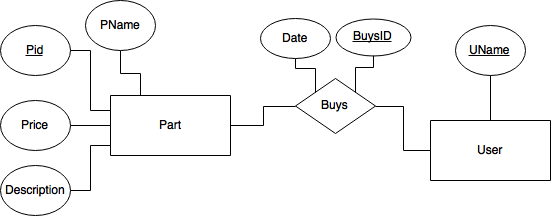
\includegraphics[width=\columnwidth]{BuysRelation.png}
\\
\\Relation: Writes
\\Attributes: Uid : int, Rid : int, Pid : int
\\Relation to user scenario: This relation occurs as described in part 1 when a account user wishes to write at most one review on a given part. Used to keep track of the Uid (user id), and Rid (review id) in relation with the Pid (part id).
\\Related Entities: Review, Account User, Part
\\
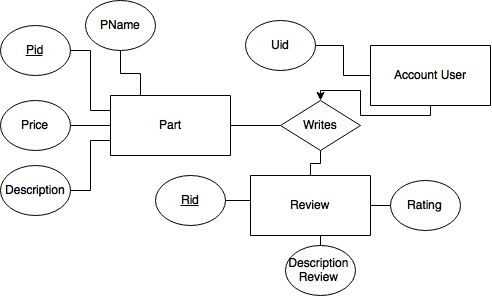
\includegraphics[width=\columnwidth]{WritesRelation.png}
\\
\\Relation: Distributes To
\\Attributes: Cid (Company id) : int, Sid (Seller id) : int
Relation to user scenario: When a user wishes to buy a part, they are given a link to the sellers which distribute the part, in order for them to distribute to the users, companies must first distribute the part to each seller. Each company distributes their part to atleast one seller to then sell that part.
\\Related Entities: Company, Seller
\\
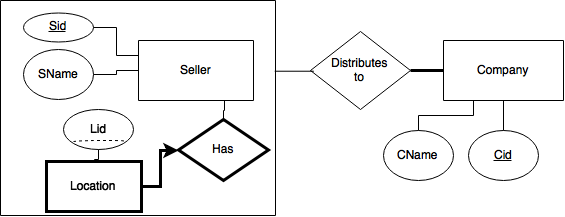
\includegraphics[width=\columnwidth]{distributesrelation.png}
\\
\\Relation: Sold By
\\Attributes: Sid : int, Pid : int
\\Relation to user scenario: Similar to the previous scenario, when an account user makes a purchase they are given a link to the seller of their choosing. This relation relates all sellers to products they sell, and all sellers who sell a certain part. 
\\Related Entities: Seller, Part
\\
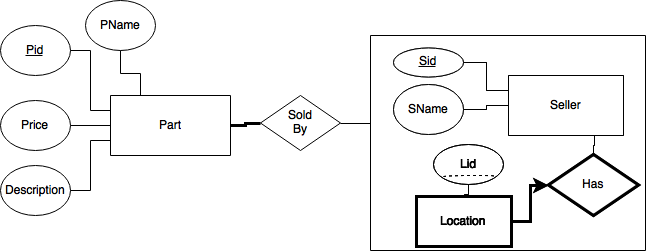
\includegraphics[width=\columnwidth]{soldbyrelation.png}
\\
\\Relation: Manufactures
\\Attributes: Pid : int, Cid : int
\\Relation to user scenario: When a company releases a new part, this relation keeps track of how each part is manufactured. Each individual product in the Computer Hardware Database is manufactured by exactly one company. For example: Intel and Kingston cannot both manufacture Intel Core i7 Processors, only Intel can.
\\Related Entities: Part, Company
\\
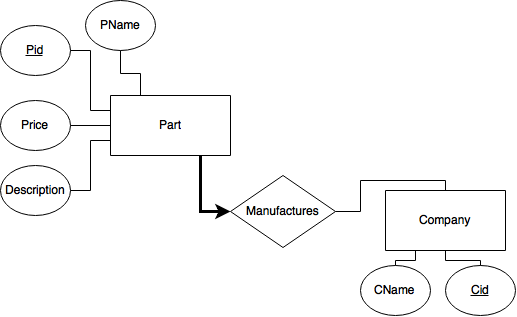
\includegraphics[width=\columnwidth]{manufacturesrelation.png}
\\
\\Relation: Has
\\Attributes: Lid : int, Sid : int
\\Relation to user scenario: When describing the Seller entity, we decided to describe it in terms of an additional relation and entity within an aggregate. Whenever a seller is called upon within a relation, the seller location will describe that seller within a unique location containing a Lid. This relation is a weak entity in that if a Seller is removed, the location describing that seller will be removed as well.
\\
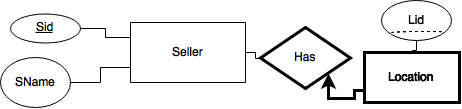
\includegraphics[width=\columnwidth]{residesrelation.png}
\\
\\Relation: Reviews
\\Attributes: Rid : int, Pid : int
\\Relation to user scenario: Each review reviews exactly 1 part. This relation keeps track of the review id and the part that it applies to. 
\\Related Entities: Part, Review
\\
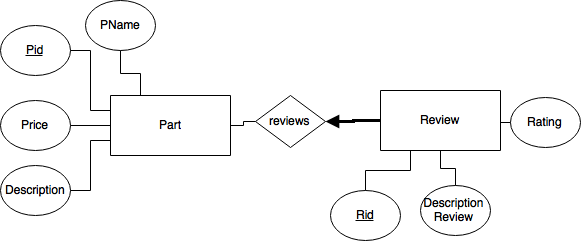
\includegraphics[width=\columnwidth]{hasrelation.png}
\\
\\Relation: is Part of
\\Attributes: Pid1 : int, Pid2 : int
\\Relation to user scenario: Each part is a component of multiple parts. In a real-world user scenario, computer parts are very complex and made up of multiple individual computer parts. We accounted for this by implementing this relation.
\\Related Entities: Part
\\
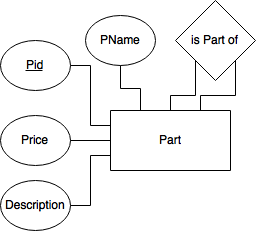
\includegraphics[width=\columnwidth]{ispartofrelation.png}
\\
\item{ The description relating this ER part (relation) as it corresponds to one or more user scenario(s): }
Please insert the description relating this ER part to user scenario(s), in here.
\end{itemize}
Please repeat that pattern for each relation.
\begin{itemize} 
\item{ The ER diagram in its entirety: }
\\
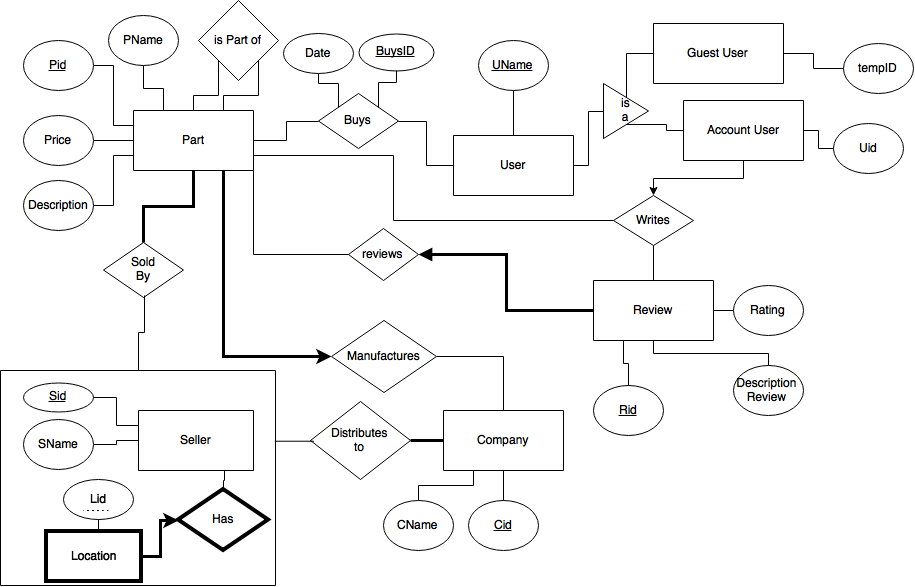
\includegraphics[width=\columnwidth]{ERDiagram.png}
\item{ The ER diagram description (corresponding to the user scenarios): }
Above is our ER diagram depicting numerous user type scenarios that could take place within our computer hardware database. In our ER diagram, we based the different user types as entities themselves, with the addition of a ''Review'' and ''Part'' entity. Having user types as entities allows us leeway for enacting our user scenarios through the use of relations of those entities. The ER diagram closely follows the user scenarios that were previously described in this report. For example, the ''User'' entity ''Buys'' a ''Part'' that is ''Sold By'' a ''Seller''. This scenario is clearly depicted in the ER diagram above and numerous other user scenarios are clearly described as well. With the addition of the entities are their potential attributes and relations to other entities. The ''Writes'' relation relates to a ''Review'' entity and a ''Account User'' entity. The ''Part'' entity is tied to six potential relations, which includes ''Buys'',''Has'', 'Manufactures'', ''is Part of'', ''Writes'' and ''Sold Buy''. Furthermore, a ''Account User'' has the ability to ''Write'' a ''Review'' or ''Buy'' a ''Part''. Lastly, our ''Company'' entity has a primary purpose of ''Distributing to'' the ''Seller'' entity, from whom a ''Part'' is ''Sold by''. In regards to the attributes we have chosen for each entity, all entities contain at least one primary key that helps to distinguish themselves from other entities. Overall, we tried to compose a database design that was easy to follow yet completes its task quickly and without problems. All user scenarios are clearly described in this single ER diagram in such a way that connects each of our entities in a logical and reasonable manner.
\\
\item{ The integrity constraints defined in the ER diagram: }
Each part is sold by atleast one seller, each company distributes to atleast one seller that resides at a particular location, each part is manufactured by exactly one company, a covering constraint indicating that each user type must either be an ''Account User'' or a ''Guest User'', a weak entity amongst a ''Location'' that only exists if there is a ''Seller'' entity and each account user writes at most one review for a given part. Additionally, each ''Review'' ''reviews'' exactly one ''Part''. 
\begin{itemize} 
\item{ Integrity Constraint: }
Each part is sold by at least one seller.
\item{ The description and justification of the integrity constraint: }
The first integrity constraint we included in our ER diagram relates to the ''Part'' entity and the ''Sold By'' relation. In order to make logical sense of our ER diagram, we created this constraint with the fact that  a part is sold by atleast one seller. A single part can be sold by multiple sellers. 
\end{itemize}
\begin{itemize} 
\item{ Integrity Constraint: }
Each company distributes to at least one seller that resides in a location (aggregate).
\item{ The description and justification of the integrity constraint: }
The second integrity constraint we included in our ER diagram relates to the ''Company'' entity and the ''Distributes to'' relation. We constructed this constraint with the idea that at a Company distributes their manufactured part to atleast one ''Seller''. A  company should be able to distribute their part to a collection of sellers. 
\end{itemize}
\begin{itemize} 
\item{ Integrity Constraint: }
Each part is manufactured by exactly one company.
\item{ The description and justification of the integrity constraint: }
The third integrity constraint we included in our ER diagram relates to the ''Part'' entity and the ''Manufactures'' relation to ''Company'. Each part in the database is manufactured by exactly one company. No identical part is manufactured by more than one company. Each company can manufacture many parts as well.
\end{itemize}
\begin{itemize} 
\item{ Integrity Constraint: }
A covering constraint indicating that each user type must either be an ''Account User'' or a ''Guest User''
\item{ The description and justification of the integrity constraint: }
In our model, we have two potential user types that have similar roles but vary in allowed attributes. As compared to account users who carry a unique Uid, guest users carry a tempID that distinguishes them from account users. By implementing an ISA relationship, we can account for both account users and guest users.
\end{itemize}
\begin{itemize} 
\item{ Integrity Constraint: }
A weak entity amongst a ''Location''. Each seller location only exists if there is a ''Seller'' entity. 
\item{ The description and justification of the integrity constraint: }
In order for there to be a seller location, a seller must exist. This indicates that the ''Location'' entity is a weak entity in the fact that a location can not exist without a seller. Each location has a seller tied to it and will be deleted if a seller is deleted from the database.  
\end{itemize}
\begin{itemize} 
\item{ Integrity Constraint: }
Each Account User writes at most one review for a given part.
\item{ The description and justification of the integrity constraint: }
In our computer hardware database design, we decided that an account user type can write a single review on a give computer part. To account for this, we drew an arrow relating the ''Review'' and ''Writes'' relationship in order to indicate this constraint. An account user should not be able to write multiple reviews on a single computer hardware part. This keeps the database free from user-review spamming and keeps the integrity of the content in our database at a high level. 
\end{itemize}
\end{itemize}
}


\subsection{Stage3 - The Implementation Stage. }\label{sec: 3 The Implementation Stage.}
%%%%%%%%%%%%%%%%%%%%%%%%%%%%%%%%%%%%%%%%%%%%%%%%%%%%%%%%%%%%%%%%%%%%%%%%%%%%%%%%%%%%%%%%%%%%%%%%%%%%%%%%%%
\textnormal{
\begin{itemize} 
	\item{The normalization step for the SQL table and the explanations/justification of the normalization step and The normalization steps for each table, along with explanations/justifications and the normalization steps for each table, along with explanations/justifications the SQL Table, including data entries }
\includegraphics[width=\columnwidth]{SQLTables1.png}
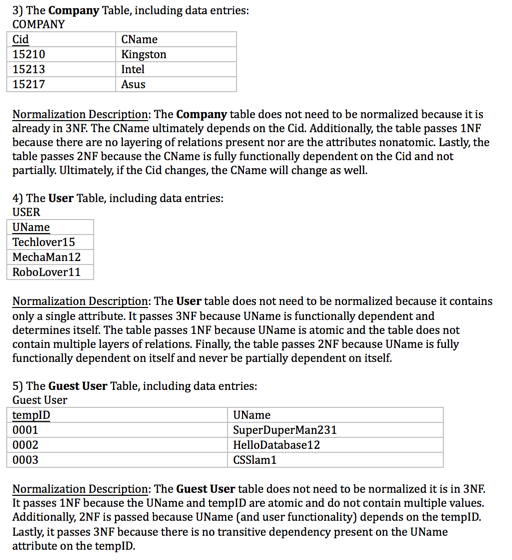
\includegraphics[width=\columnwidth]{SQLTables2.png}
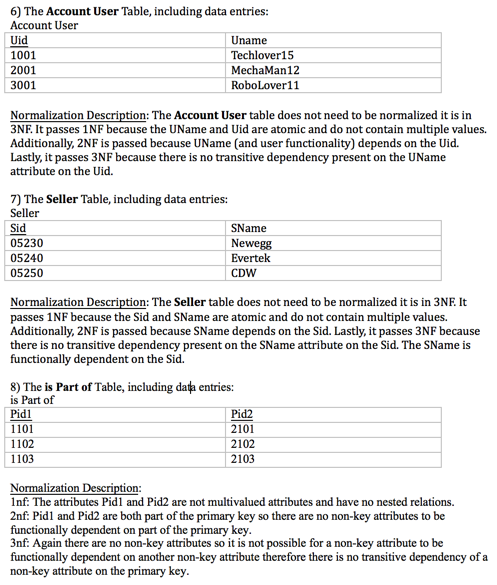
\includegraphics[width=\columnwidth]{SQLTables3.png}
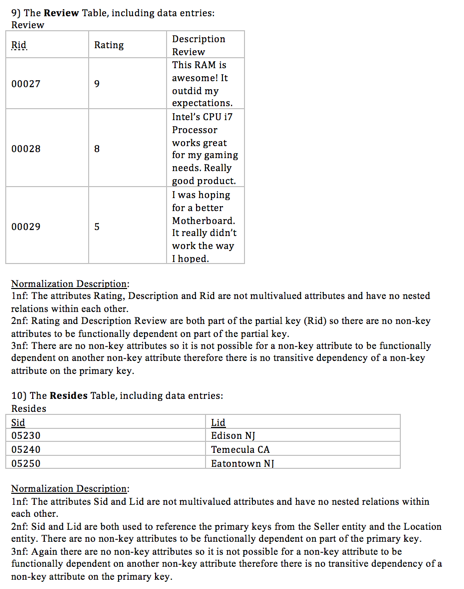
\includegraphics[width=\columnwidth]{SQLTables4.png}
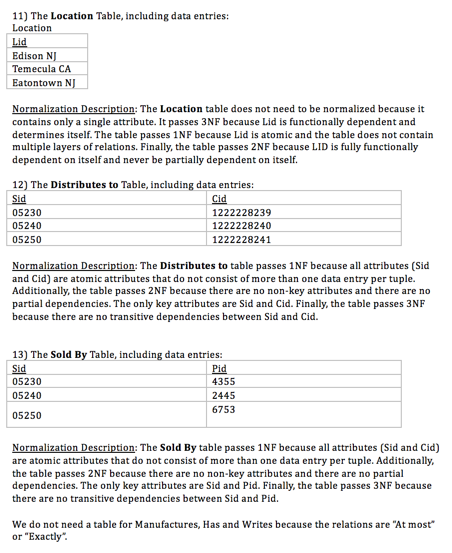
\includegraphics[width=\columnwidth]{SQLTables5.png}
\item{}
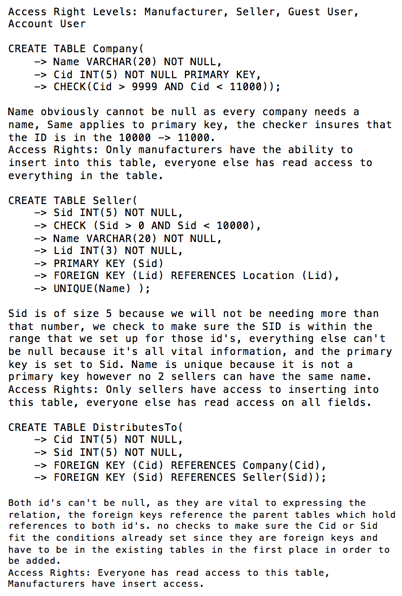
\includegraphics[width=\columnwidth]{SQLQueries1.png}
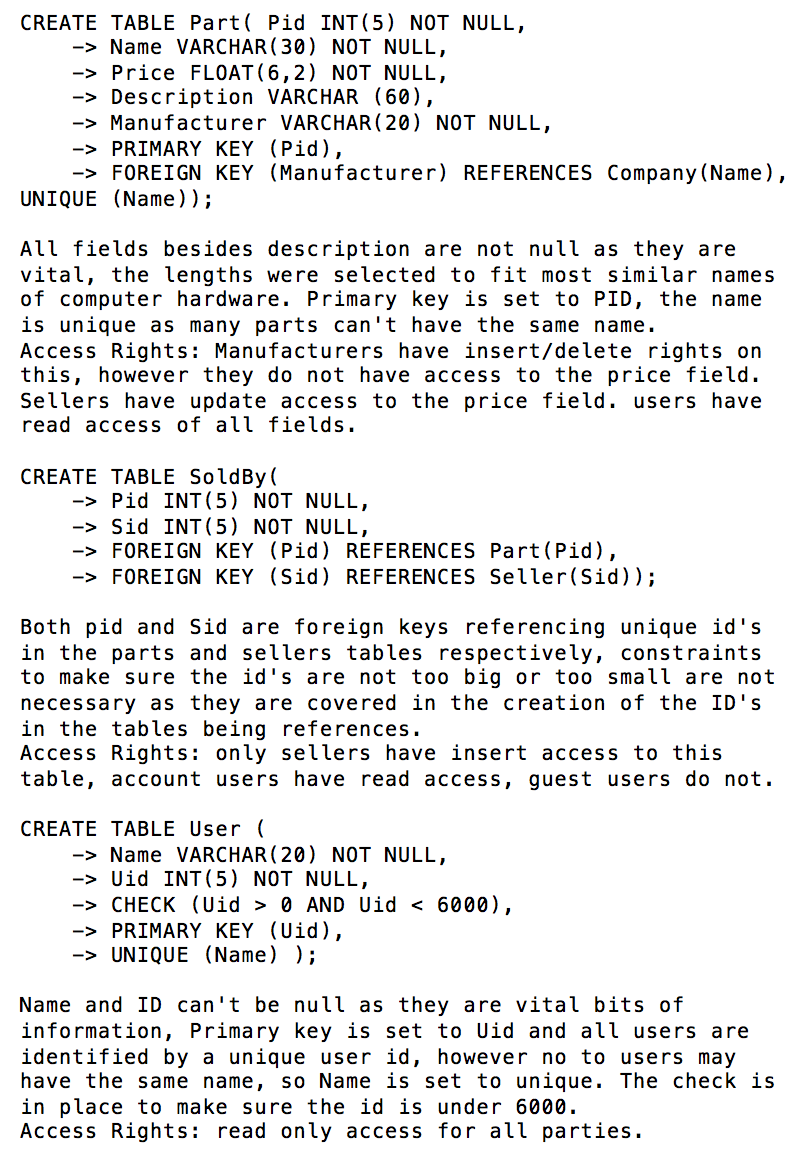
\includegraphics[width=\columnwidth]{SQLQueries2.png}
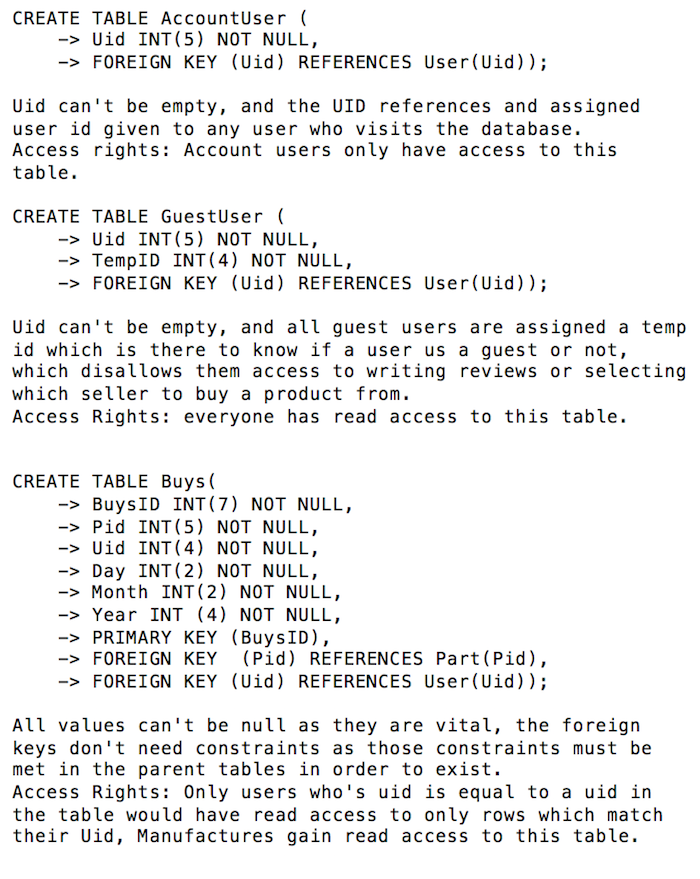
\includegraphics[width=\columnwidth]{SQLQueries3.png}
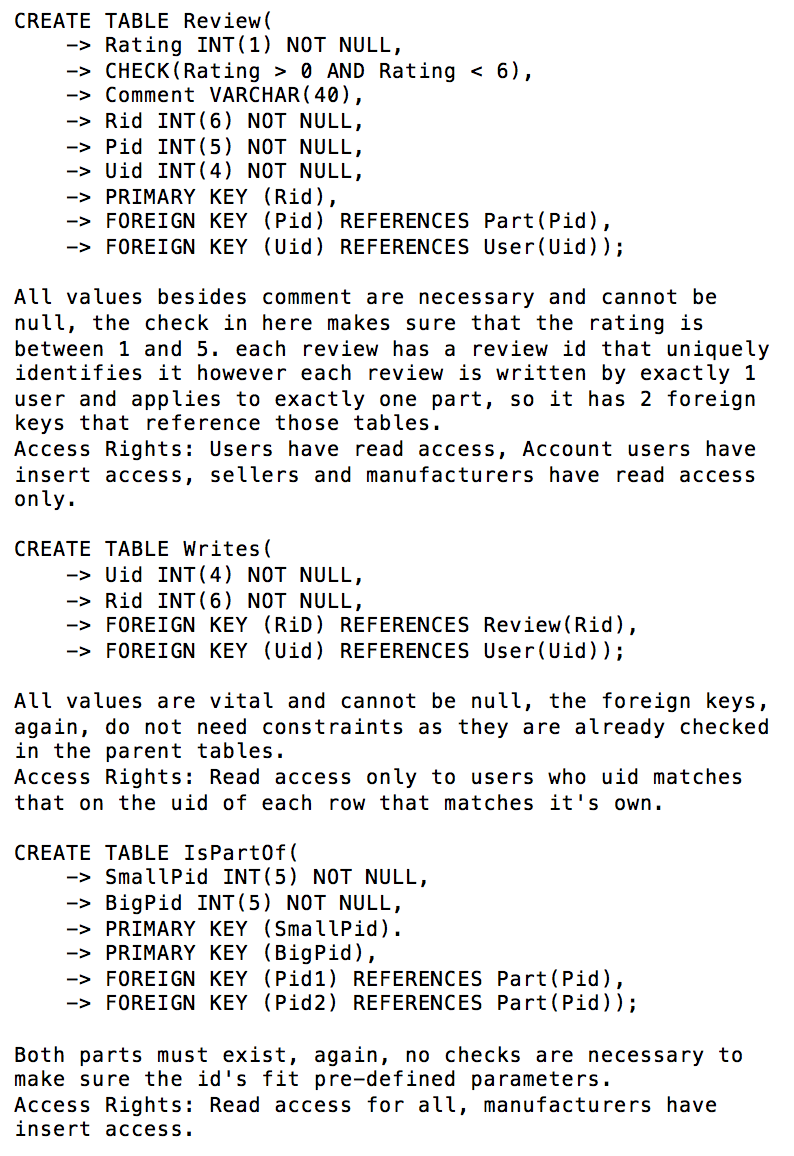
\includegraphics[width=\columnwidth]{SQLQueries4.png}
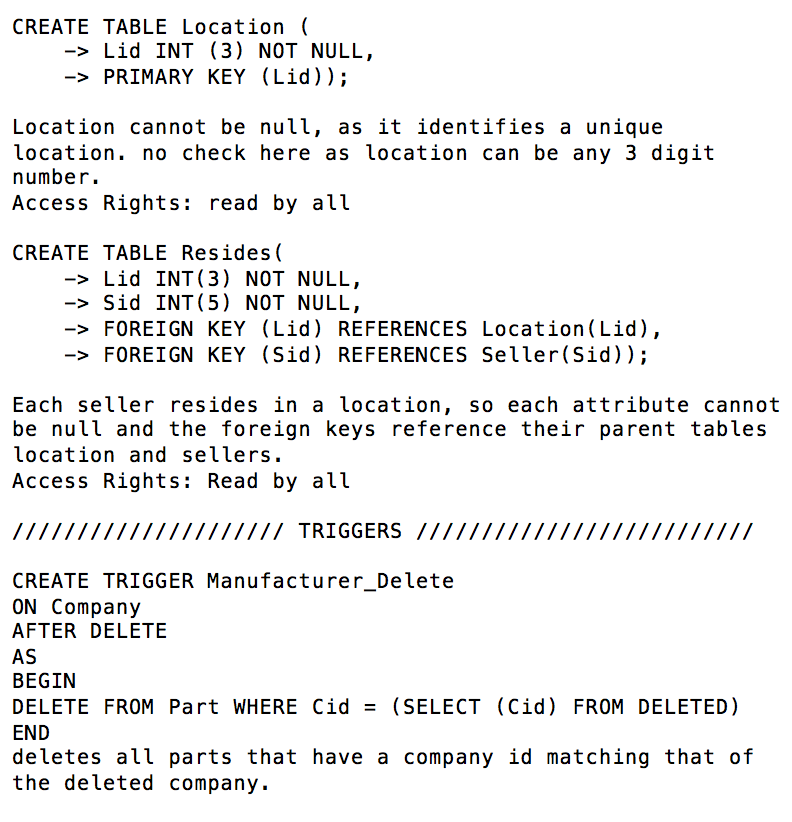
\includegraphics[width=\columnwidth]{SQLQueries5.png}
\end{itemize}
}


\subsection{Stage4 -	User Interface. }\label{sec: 4.	User Interface.}
%%%%%%%%%%%%%%%%%%%%%%%%%%%%%%%%%%%%%%%%%%%%%%%%%%%%%%%%%%%%%%%%%%%%%%%%%%%%%%%%%%%%%%%%%%%%%%%%%%%%%%%%%%
\textnormal{
\begin{itemize} 
\item{The the first SQL statement used to query the data: }
Here is a simple query to start off:\\
	SELECT * \\FROM Part P \\WHERE P.PName = "Intel Computer Stick" \\    AND P.Pid = 1337\\
	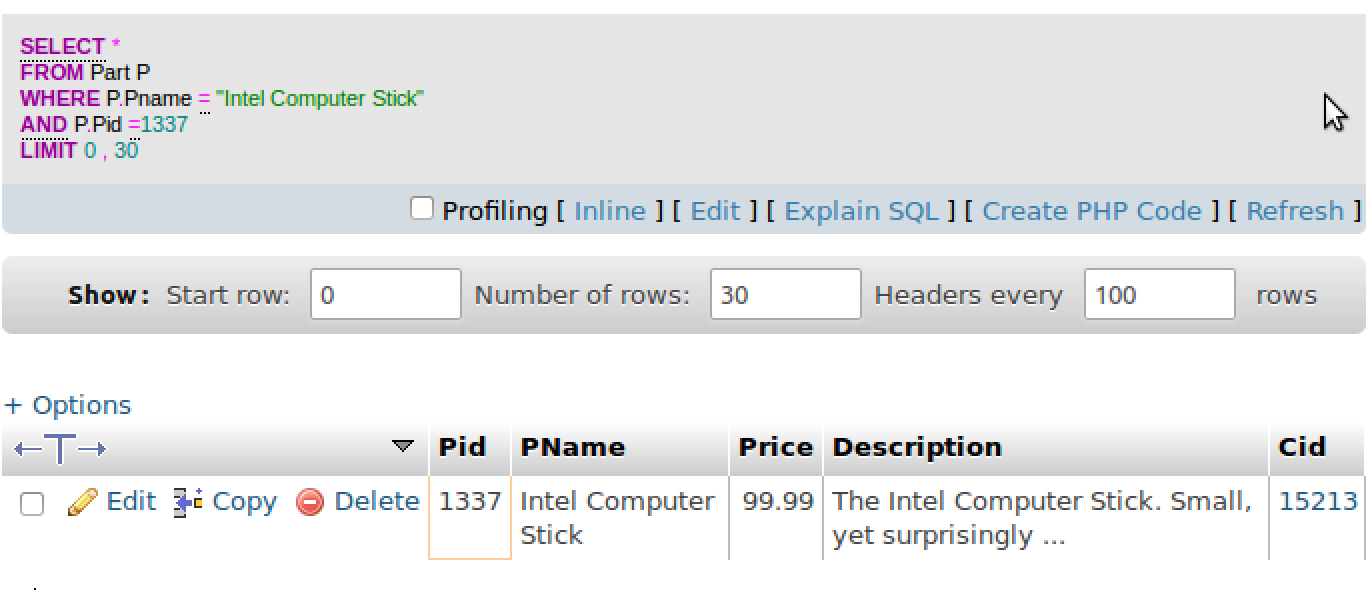
\includegraphics[width=\columnwidth]{Query1.png} 
\item{The tables taking part in the query statement (table names and headers): }
	 \begin{itemize} 
	 \item{The name of the first table taking part in the query: }
	 Part table
	  \item{The header of the table  (all attributes): }
	  Pid, PName, Price, Description, Cid
	  \item{The attributes of the table taking part in the query: }
	  PName and Pid
	 \end{itemize}
\item{The the second SQL statement used to query the data: }
	SELECT * \\FROM Part P, Buys B\\WHERE P.Pid = B.Pid\\
	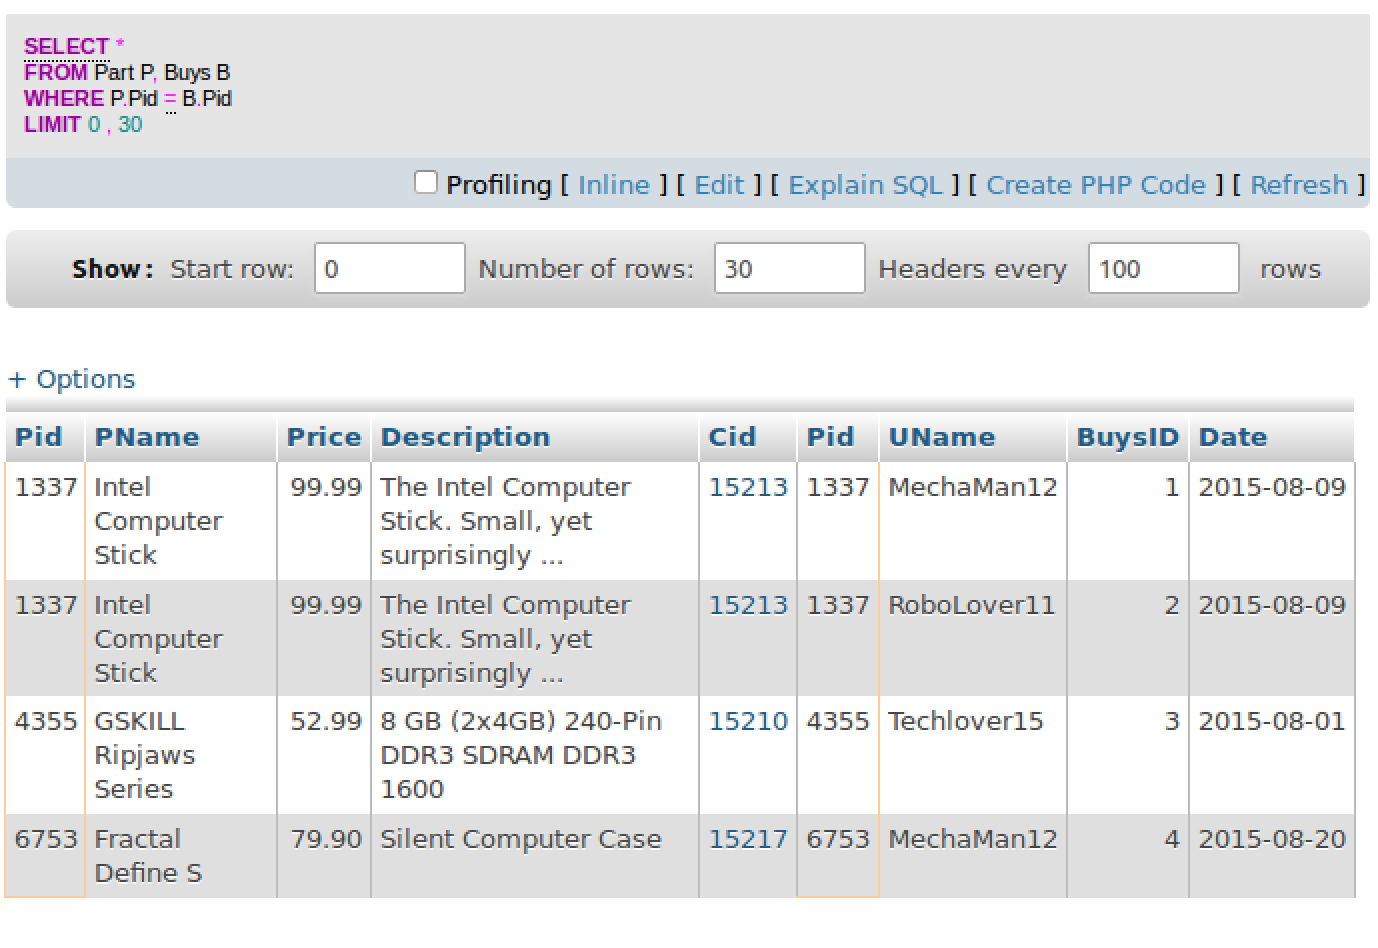
\includegraphics[width=\columnwidth]{Query2.png} 
\item{The tables taking part in the query statement (table names and headers): }
	 \begin{itemize} 
	 \item{The name of the tables taking part in the query: }
	 Part and Buys table
	  \item{The header of the table  (all attributes): }
	  Part: Pid, PName, Price, Description, Cid \\
	  Buys: Pid, UName, BuysID, Date
	  \item{The attributes of the table taking part in the query: }
	   Pid
	 \end{itemize}
	 \item{The the third SQL statement used to query the data: }
	SELECT * \\FROM Part P, Review R\\WHERE R.Rating >= 8 \\ AND P.Pid = R.Pid\\
	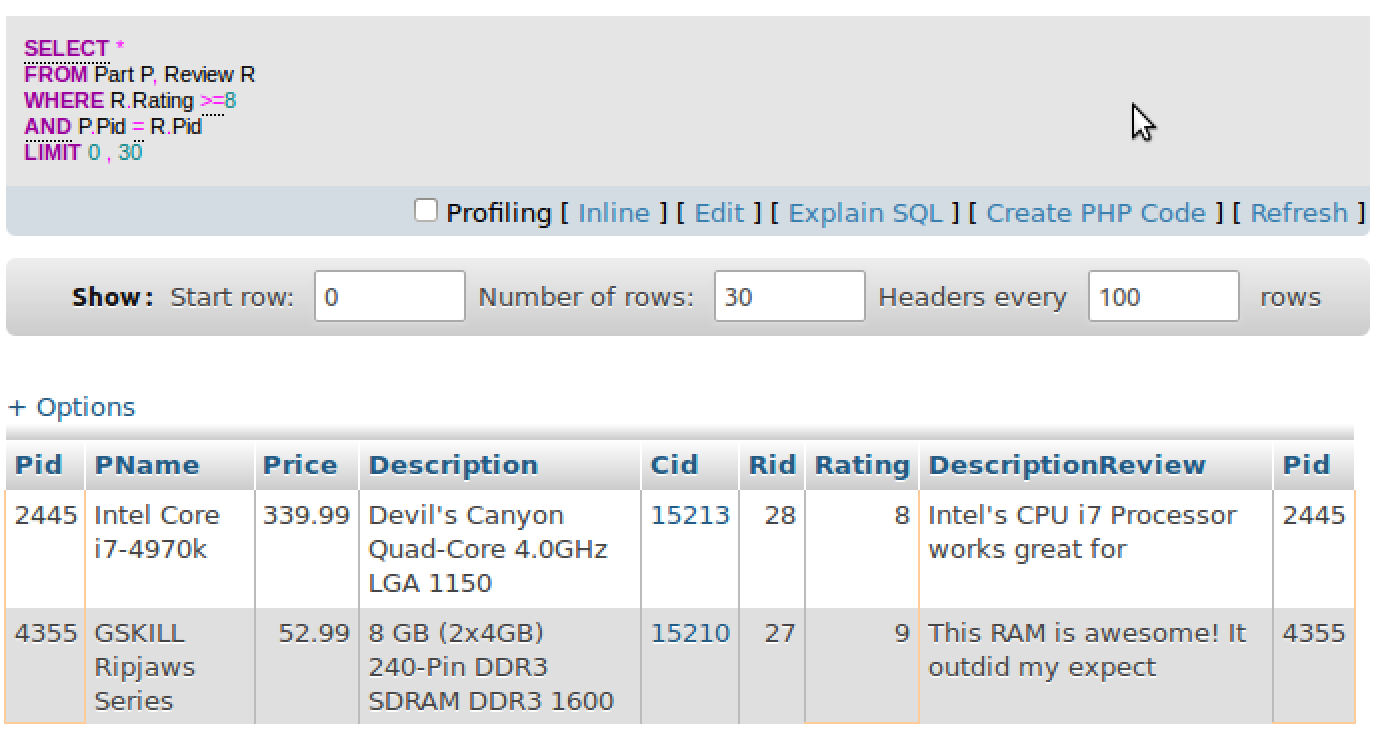
\includegraphics[width=\columnwidth]{Query3.png} 
\item{The tables taking part in the query statement (table names and headers): }
	 \begin{itemize} 
	 \item{The name of the tables taking part in the query: }
	 Part and Review table
	  \item{The header of the table  (all attributes): }
	  Part: Pid, PName, Price, Description, Cid \\
	  Review: Pid, Rid, Rating, Review Description
	  \item{The attributes of the table taking part in the query: }
	   Pid, rating
	 \end{itemize}
	 \item{The the fourth SQL statement used to query the data: }
	SELECT S.SName, P.PName \\FROM Seller S, Part P\\WHERE P.Price >= 99.99\\
	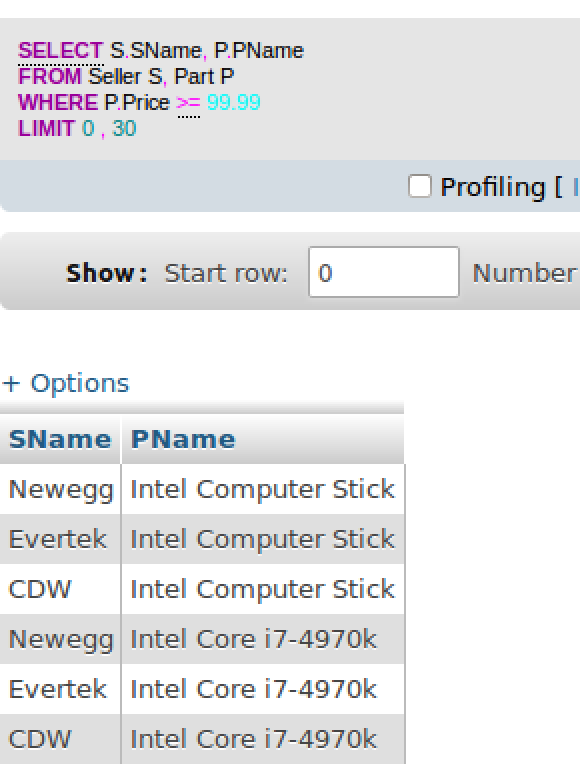
\includegraphics[width=\columnwidth]{Query4.png} 
\item{The tables taking part in the query statement (table names and headers): }
	 \begin{itemize} 
	 \item{The name of the tables taking part in the query: }
	 Seller and Part tables
	  \item{The header of the table  (all attributes): }
	  Part: Pid, PName, Price, Description, Cid \\
	  Seller: Sid, SName
	  \item{The attributes of the table taking part in the query: }
	   SName and PName
	 \end{itemize}
	 \item{The the fifth SQL statement used to query the data: }
	SELECT L.Lid \\FROM Seller S, Location L\\WHERE S.SName = ''Newegg'' OR S.SName = ''Evertek'' AND S.Sid = 5250\\
	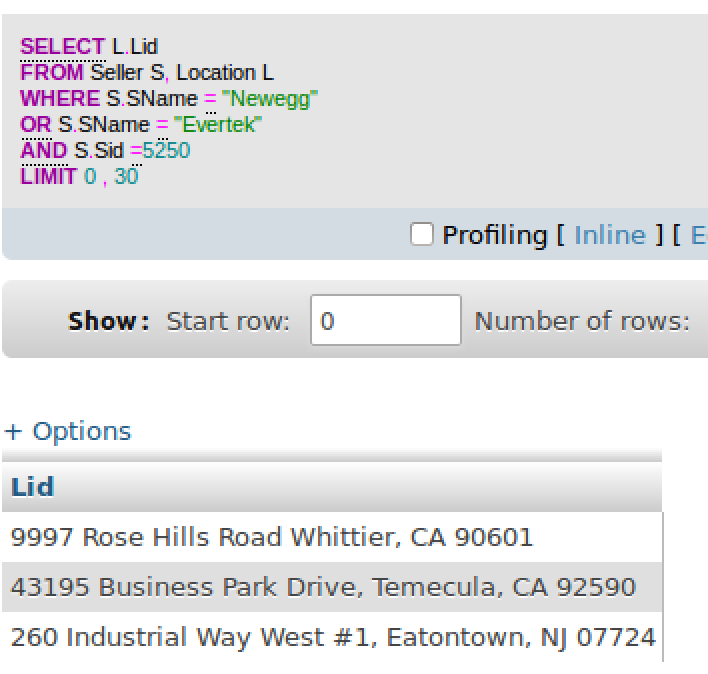
\includegraphics[width=\columnwidth]{Query5.png} 
\item{The tables taking part in the query statement (table names and headers): }
	 \begin{itemize} 
	 \item{The name of the tables taking part in the query: }
	 Seller and Location table
	  \item{The header of the table  (all attributes): }\\
	  Location: Lid \\
	  Seller: Sid, SName
	  \item{The attributes of the table taking part in the query: }
	   Lid
	 \end{itemize}
\item{}
	The error messages popping-up when users access and/or updates are denied (along with explanations and examples):
	\begin{itemize} 
	\item{The first error message: }
	\\CREATE command denied to user Account User
		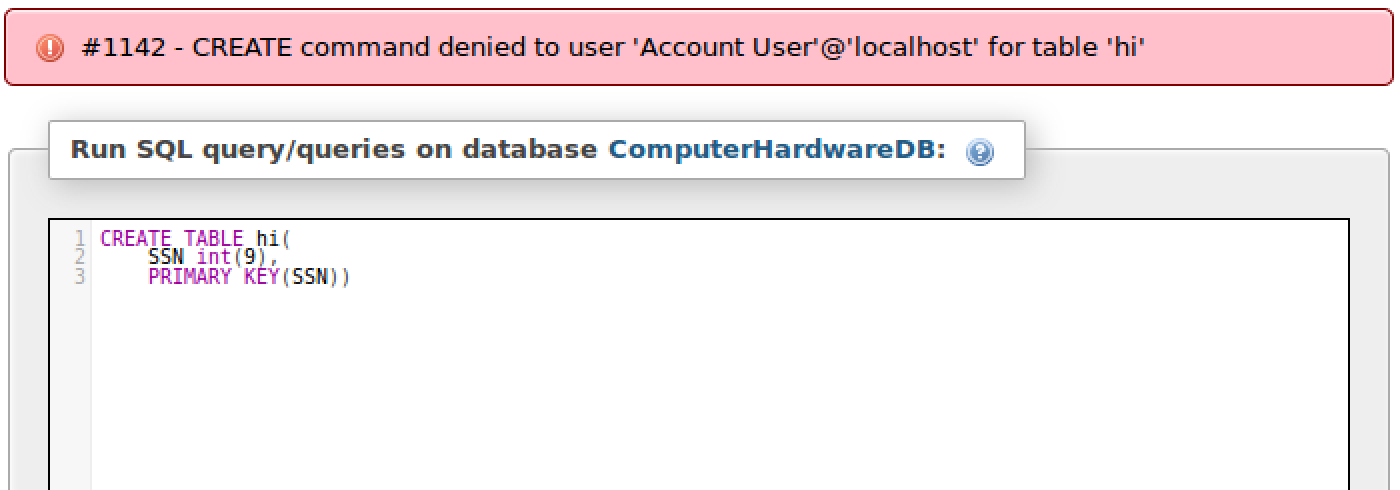
\includegraphics[width=\columnwidth]{Access1.png}
	\item{The error message explanation (upon which violation does it take place): }
	The user does not have the access rights for creating a table. 
	\item{The error message example according to user(s) scenario(s): }
	This account user accessing the Computer Hardware DB tried creating a table in the database. Account users, however, do not have access rights to do so. This account user must have mixed up his command with INSERT, a command which Account users are allowed access when inserting a rating and description review for the Reviews entity.\\
	Example:\\
	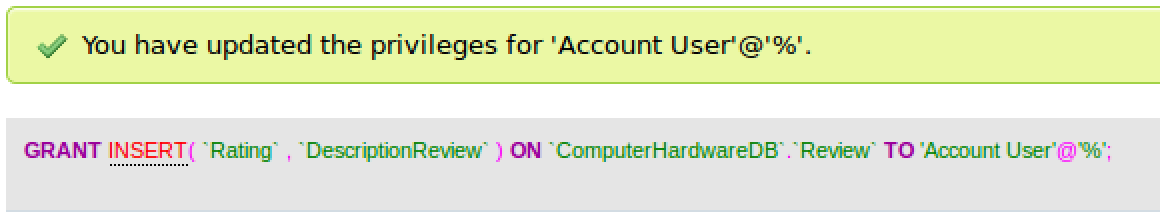
\includegraphics[width=\columnwidth]{Access2-1.png}
	 \end{itemize}
	\begin{itemize} 
	\item{The second error message: }
	\\INSERT command denied to user Guest User
		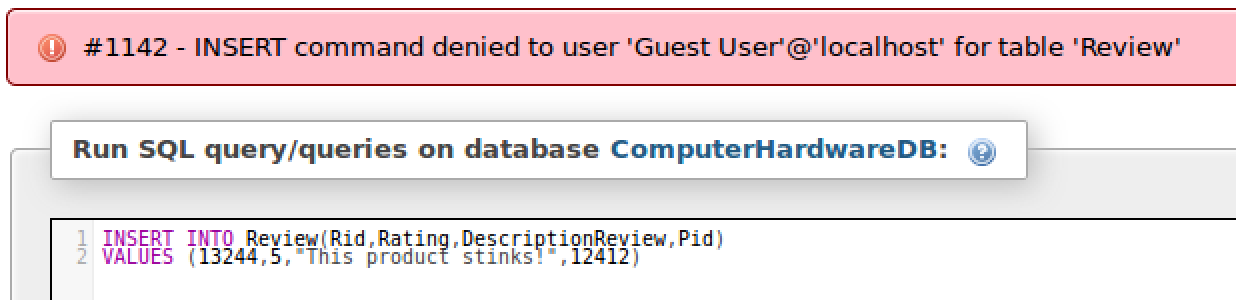
\includegraphics[width=\columnwidth]{Access2-2.png}
	\item{The error message explanation (upon which violation does it take place): }
	The user does not have the access rights for inserting into the database. 
	\item{The error message example according to user(s) scenario(s): }
	This guest user accessing the Computer Hardware DB tried inserting into the Review entity. Guest users, however, do not have access rights to do so. Guest user cannot write reviews or rate reviews like account users.
	 \end{itemize}
	 \begin{itemize} 
	\item{The third error message: }
	\\ALTER command denied to user Account User
		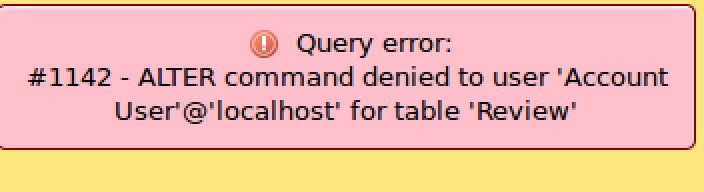
\includegraphics[width=\columnwidth]{Access3.png}
	\item{The error message explanation (upon which violation does it take place): }
	The user does not have the access rights for altering a table in the database. 
	\item{The error message example according to user(s) scenario(s): }
	This account user accessing the Computer Hardware DB tried to alter a table in the database. Account users, however, do not have access rights to do so. Account user cannot alter pre-existing attribute specifications in a table.
	 \end{itemize}
	 	 \begin{itemize} 
	\item{The fourth error message: }
	\\DELETE command denied to user Seller User
		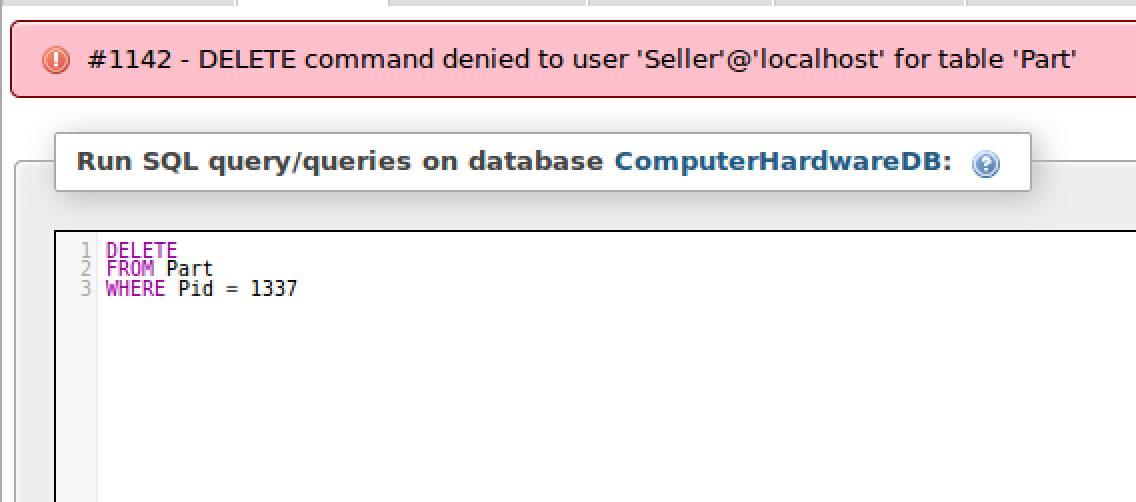
\includegraphics[width=\columnwidth]{Access4.png}
	\item{The error message explanation (upon which violation does it take place): }
	The user does not have the access rights for deleting information from a table in the database. 
	\item{The error message example according to user(s) scenario(s): }
	This seller accessing the Computer Hardware DB tried to delete a Pid from a table in the database. Seller users should not have access rights for deleting product information on a company's part. Only Company users should be able to remove their own information on a given part.
	 \end{itemize}
	 \begin{itemize} 
	\item{The fifth error message: }
	\\DROP command denied to user Company User
		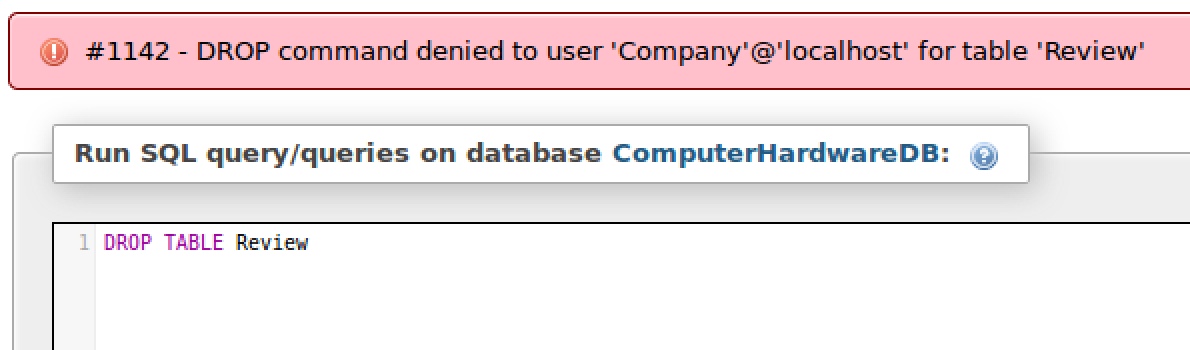
\includegraphics[width=\columnwidth]{Access5.png}
	\item{The error message explanation (upon which violation does it take place): }
	The user does not have the access rights for dropping an entire table from the database.
	\item{The error message example according to user(s) scenario(s): }
	This company user accessing the Computer Hardware DB tried to drop the Review table from the database. Company users, as well as all users of the database (with the exception of the DBA) should not have access rights for dropping entire tables from the database. The company user may have wanted to delete a review on their product that an account user did not like. Although it is frustrating to see bad reviews on a product one may have created, a prestigious company such as Intel should not take it to heart and rather learn from their potential falters. Ultimately, company users cannot and should not drop review information on their products.
	 \end{itemize}
\item{}
	The error messages corresponding to the integrity constraints violations (along with explanations and examples).
	\begin{itemize} 
	\item{The first error message: }
	Duplicate entry '4124' for key 'PRIMARY'\\
	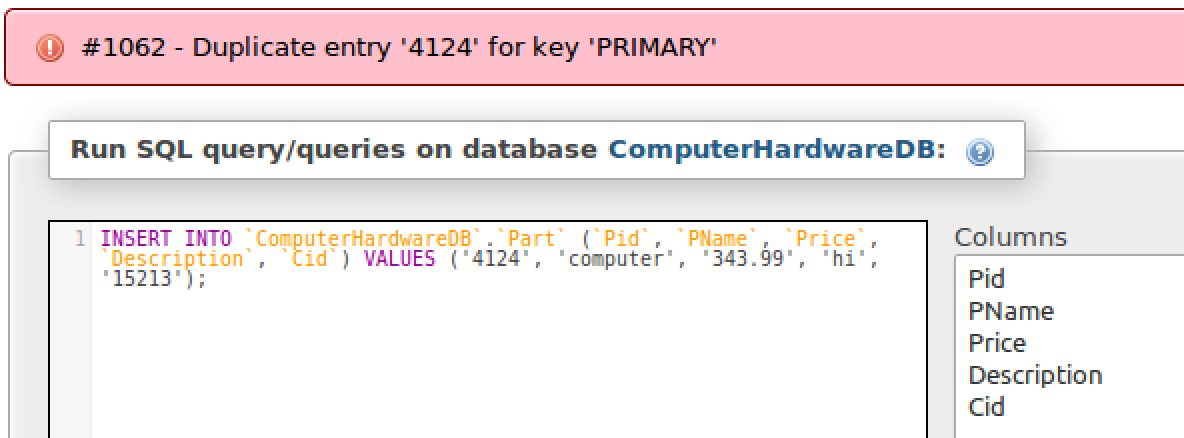
\includegraphics[width=\columnwidth]{integrity1.png}
	\item{The error message explanation (upon which violation does it take place): }
	When trying to INSERT a duplicate primary key for Pid, the system stops the command with a duplicate primary key constraint.  
	\item{The error message example according to user(s) scenario(s): }
	In order to ensure that changes made to the database do not result in loss of data and consistency, our database holds PRIMARY keys. These keys (such as Pid) allow our products in Part to be unique and have individual characteristics from all parts being added to the database. In the case if a seller tried to INSERT a duplicate part by accident in their retail system, the database system would catch it and save the seller time and money trying to find the root cause that is throwing off their inventory calculations. Having duplicate part ids can most definitely throw off a inventory database, and it is accounted for in our database.
	 \end{itemize}
	 	\begin{itemize} 
	\item{The second error message: }
	Cannot delete or update a parent row: a foreign key constraint fails\\
	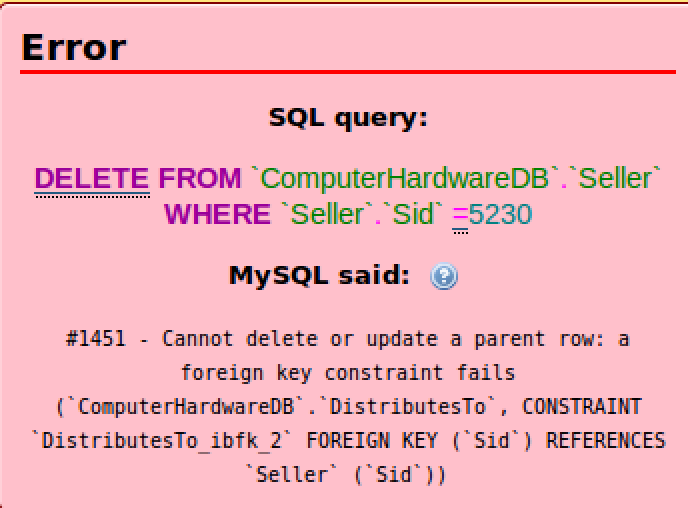
\includegraphics[width=\columnwidth]{integrity2.png}
	\item{The error message explanation (upon which violation does it take place): }
	When trying to DELETE a seller tuple from the database, a FOREIGN key constraint is thrown.
	\item{The error message example according to user(s) scenario(s): }
	In order to ensure that changes made to the database do not result in loss of data and consistency, our database holds FOREIGN keys. These keys allow our tables and entities within the database to be interconnected. In this example regarding the error message above, a person using the database, most likely a seller user, tried to delete their seller information from the database. This violates the database because information regarding seller id (Sid) is already linked to Companies through relation Manufactures as well as Part through relation SoldBy. This would throw off the database entries for multiple entities and relationships since they are all connected through use of foreign keys.
	 \end{itemize}
\item{}
	The error messages corresponding to the data range constraints violations (along with explanation).
	\begin{itemize} 
	\item{The first error message: }
	Column 'Pid' cannot be null\\
	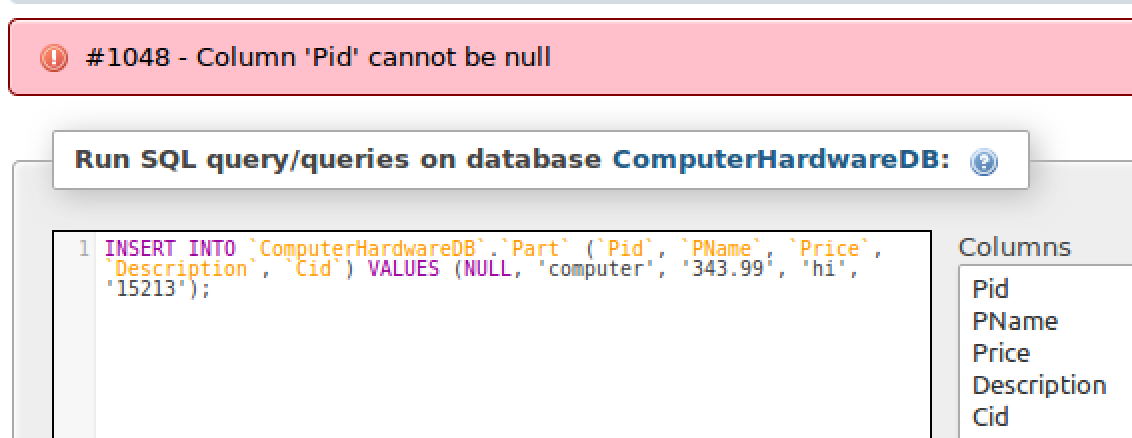
\includegraphics[width=\columnwidth]{datarange1.png}
	\item{The error message explanation (upon which violation does it take place): }
	For each PRIMARY key in the database, the value of it cannot be NULL. This would allow no uniqueness for an entity if it were given a NULL value. 
	\item{The error message example according to user(s) scenario(s): }
	An example where this error message might arise could be when a seller does not know the product id (Pid) initially but wants to insert its price, description and name. The seller cannot include NULL as information for Pid because it is a PRIMARY key. There would be no way of referencing that part if it was given a NULL value. 
	 \end{itemize}
	 	\begin{itemize} 
	\item{The second error message: }
	Out of range value for column 'Price' at row 1\\
	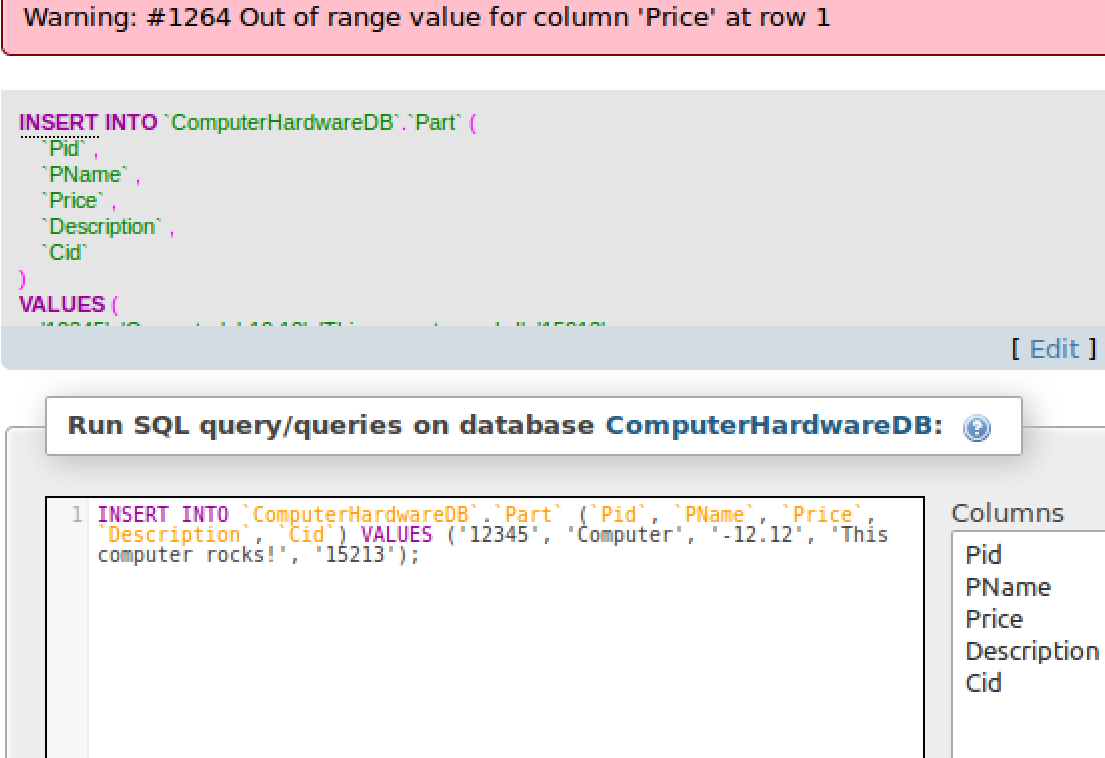
\includegraphics[width=\columnwidth]{datarange2.png}
	\item{The error message explanation (upon which violation does it take place): }
	For INT and FLOAT values in the database, they must be regarded as UNSIGNED values. There should be no negative values inserted into the database. 
	\item{The error message example according to user(s) scenario(s): }
	Most likely, the seller selling this part made a typo in the computer hardware database. A price cannot and should not be listed as a negative float value. 
	 \end{itemize}
\begin{itemize} 
	\item{The third error message: }
	Data truncated for column 'PName' at row 1\\
	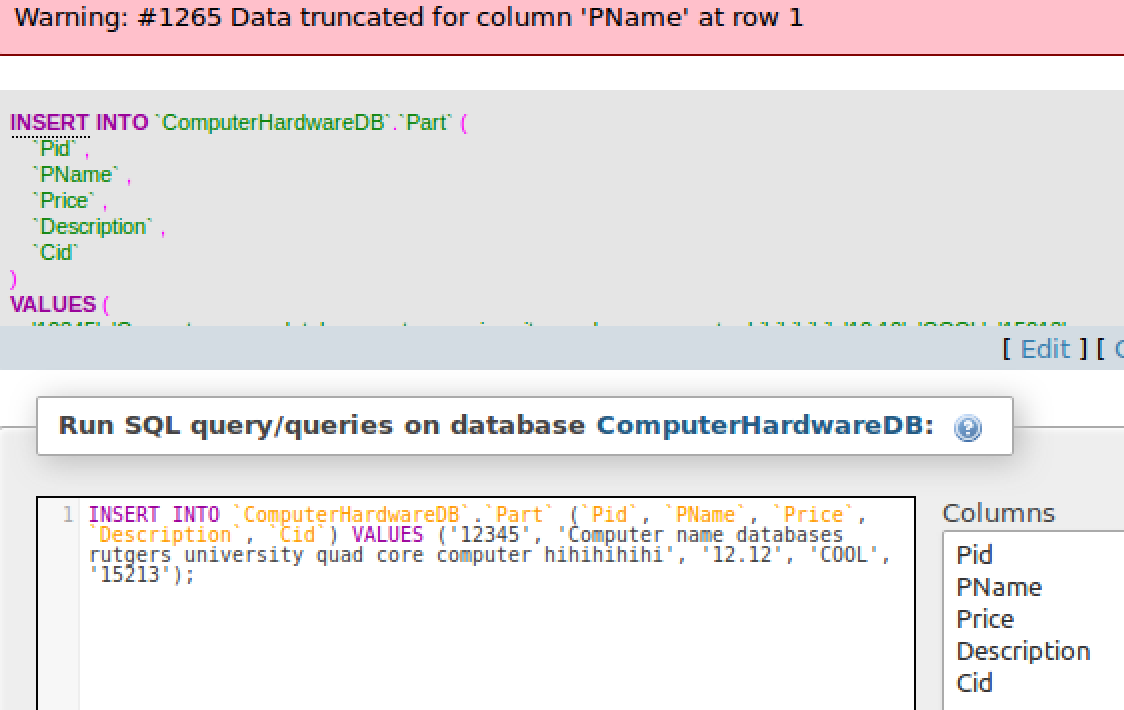
\includegraphics[width=\columnwidth]{datarange3.png}
	\item{The error message explanation (upon which violation does it take place): }
	For each product name in the Part entity, there is a limit to how long a PName can be. The error is throw because the PName is longer than varchar(30).
	\item{The error message example according to user(s) scenario(s): }
	For all varchar fields in the database, there is a certain limit to the amount of characters one can type for that attribute. This data-range constraint is to allow concise descriptions of each product name. We want to create a simple yet effective environment for our account users and guest users, and by making product descriptions clear and concise, we can achieve this. The database will automatically truncate the data if too long, hinting this to the seller/company to fix and alter immediately. 
	 \end{itemize}
\begin{itemize} 
	\item{The fourth error message: }
	Out of range value for column 'Price' at row 1\\
	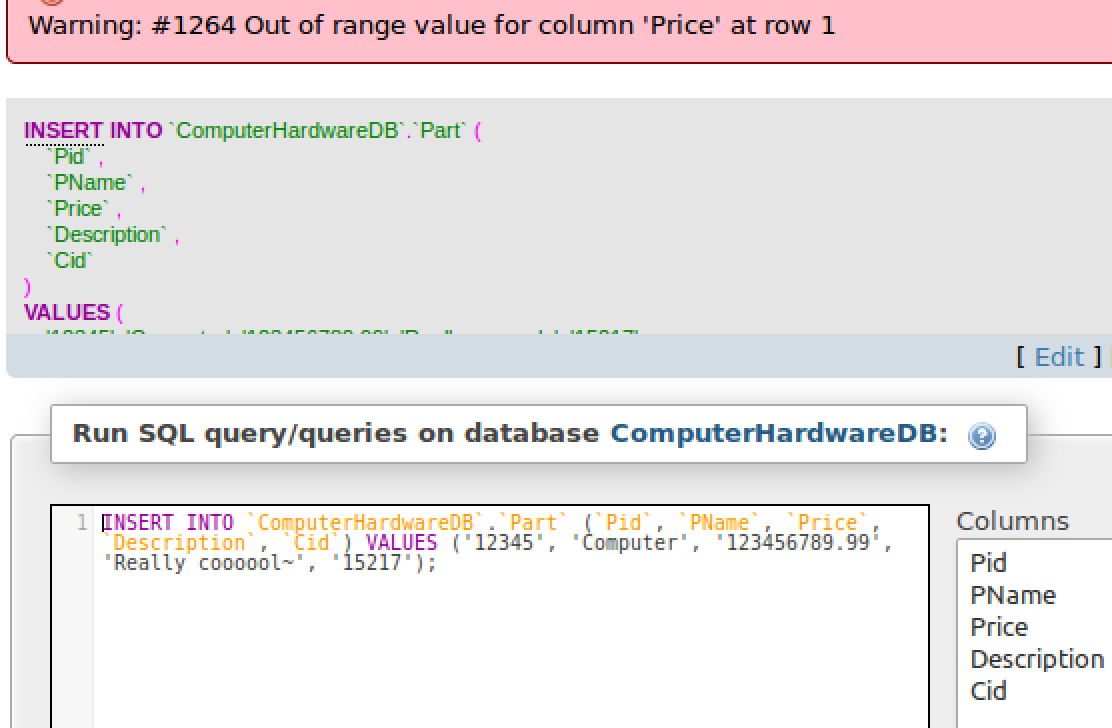
\includegraphics[width=\columnwidth]{datarange4.png}
	\item{The error message explanation (upon which violation does it take place): }
	The price of a product cannot exceed one million dollars in our database. Data that is larger than the specified data type will cause issues if not notified and dealt with immediately. We have accounted for this by adding a data-range constraint for the price field in the part entity through use of float(6,2). 
	\item{The error message example according to user(s) scenario(s): }
	 An example where this error might be thrown is when a seller lists the price of a part to be that greater than 999999.99. We do not want to deal with products greater than this value because it is simply a lot of money to deal with and there lies a lot more pressure on the database to keep the integrity and security of each transaction. If our database were to go through increased enhances involving data and transaction security, we would most definitely deal with such a fit. 
	 \end{itemize}
\item{The header of the views created in order to facilitate data accesses:}
\begin{itemize} 
	\item{The first view created: }\\
	Selects to view the part name, description, price, rating and description review.
	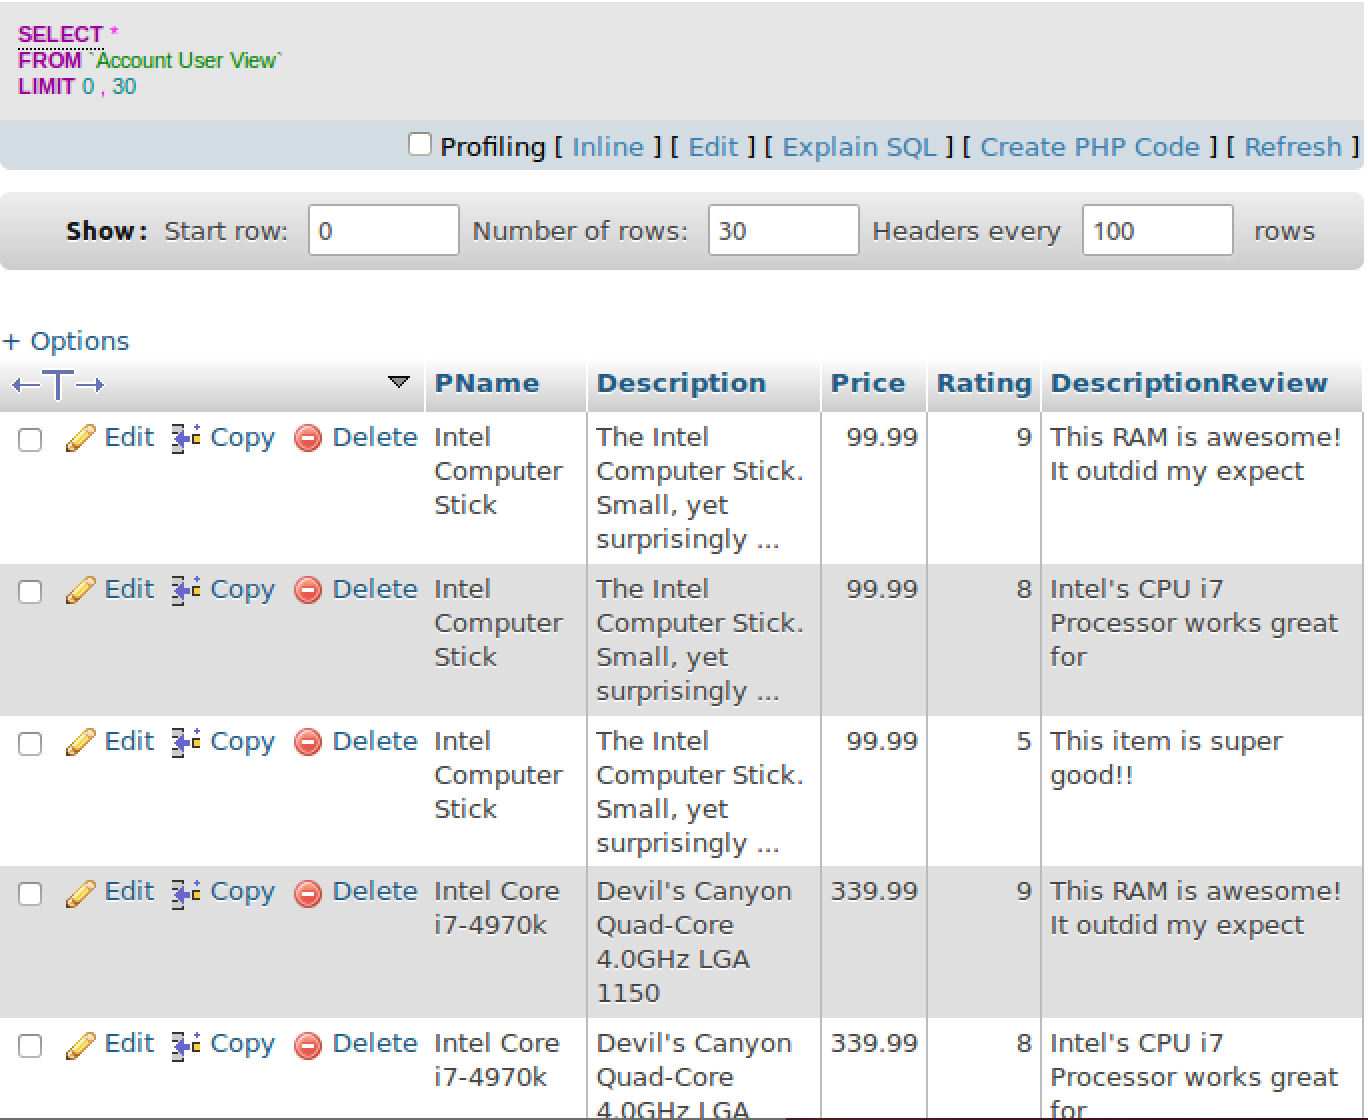
\includegraphics[width=\columnwidth]{view1.png}
	\item{The view justification: }
	This view was created with the Account User in mind. In order to make it simple for account users to make their purchase decisions, we created a view that shows all information regarding each part as well as reviews and ratings on that part. 
	\item{The tables taking part in the view and the specific attributes taking part in the view: }
	\begin{itemize} 
		\item{The table names: }
		Part and Review tables.
		\item{The table headers (all attributes): }\\
		Part: Pid, PName, Description, Price, Cid\\
		Review: Rid, Rating, DescriptionReview, Pid
		\item{The table attributes that take part in the view: }
		Part: PName, Description, Price\\
		Review: Rating, DescriptionReview
	\end{itemize}
	\item{The SQL statement used for creating the view: }
	SELECT P.Pname, P.Description, P.Price, R.Rating, R.DescriptionReview\\
	FROM Part P, Review R\\
%	\item{The trigger built upon those views (if any): }
%	Please insert the triggers as follows.
%	\begin{itemize} 
%		 \item{The trigger: }
%		Please insert the trigger in here.
%		 \item{The trigger justification (explanation, correlating it to user scenario(s)): }
%		Please insert the justification in here.
 %	\end{itemize}
 %	Please repeat for every trigger existing in the view.
\end{itemize}
\begin{itemize} 
	\item{The second view created: }\\
	Selects to view all of Intel's seller distributors of their products.\\
	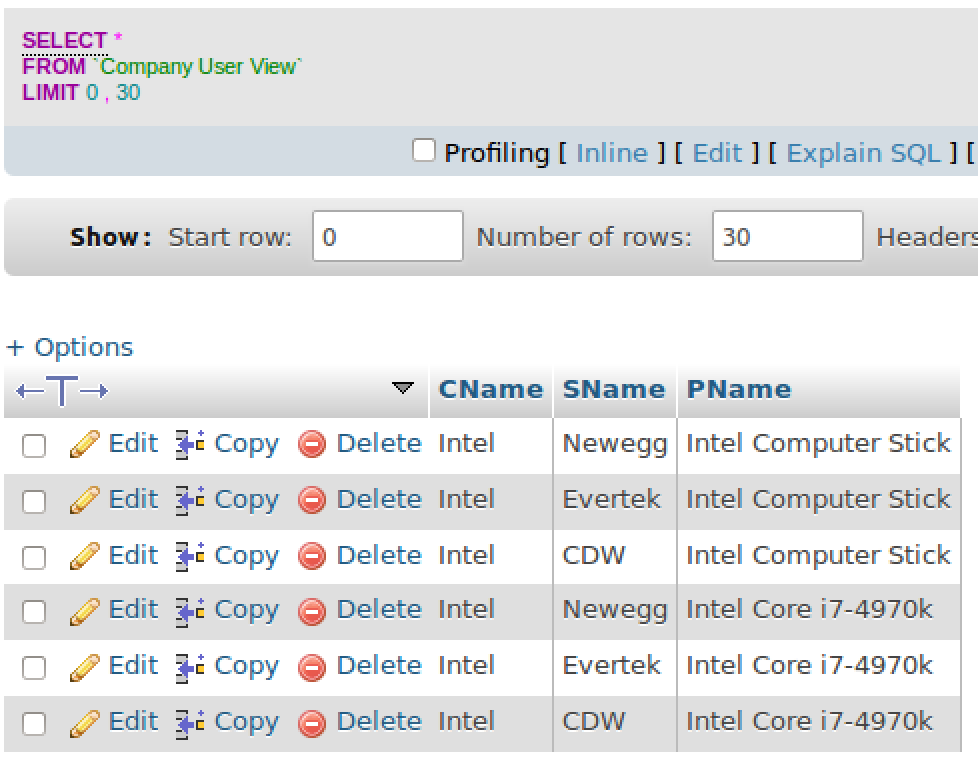
\includegraphics[width=\columnwidth]{view2.png}
	\item{The view justification: }
	This view was created with the Company User in mind. In order to keep track of their distribution of products, companies can create a view that allows them to see products they are currently distributing to different sellers.
	\item{The tables taking part in the view and the specific attributes taking part in the view: }
	\begin{itemize} 
		\item{The table names: }
		Company, Seller and Part tables.
		\item{The table headers (all attributes): }\\
		Company: Cid, CName\\
		Part: Pid, PName, Description, Price, Cid\\
		Seller: Sid, SName
		\item{The table attributes that take part in the view: }
		Company: CName\\
		Part: PName\\
		Seller: SName
	\end{itemize}
	\item{The SQL statement used for creating the view: }
	SELECT C.CName, S.SName, P.PName\\
	FROM Company C, Seller S, Part P\\
	WHERE C.CName = ''Intel'' AND C.Cid = P.Cid
%	\item{The trigger built upon those views (if any): }
%	Please insert the triggers as follows.
%	\begin{itemize} 
%		 \item{The trigger: }
%		Please insert the trigger in here.
%		 \item{The trigger justification (explanation, correlating it to user scenario(s)): }
%		Please insert the justification in here.
 %	\end{itemize}
 %	Please repeat for every trigger existing in the view.
\end{itemize}
%Please, in case you have more than one view, repeat that pattern for each view.
\end{itemize}
}


\bibliographystyle{IEEEtran}
%\bibliography{IEEEabrv,bib_queyroi_abello2013}
%\bibliography{bib_queyroi_abello2013}

\end{document}


